\documentclass[xcolor={dvipsnames}]{beamer}
\usepackage{color, colortbl}
\usepackage[ngerman,english]{babel}
\usepackage[T1]{fontenc}
\usepackage{lmodern}
\usepackage[compatibility=false]{caption}
\usepackage{subcaption}
\usepackage{tikz}
\usepackage{textgreek}
\usepackage{tabularx}
\usepackage{booktabs}
\usepackage{xspace,multicol}
\usepackage{siunitx}
\usepackage{appendixnumberbeamer}
\usepackage[absolute,overlay]{textpos} %for positioning the logos where I want


\usepackage{animate}
\usepackage{multimedia}
\usepackage{fixltx2e}
\usepackage{multicol}
\usepackage{multirow}
\usepackage{comment}
\DeclareSIUnit\year{yr}
\DeclareSIUnit\micron{\micro\metre}
\DeclareSIUnit\mrad{\milli\rad}
\DeclareSIUnit\gauss{G}
\DeclareSIUnit\nb{\nano\barn}
\DeclareSIUnit\pb{\pico\barn}
\DeclareSIUnit\fb{\femto\barn}

\newcommand{\electron}{e$^-$\xspace}
\newcommand{\positron}{e$^+$\xspace}
\newcommand{\murm}{%
  \ifmmode
    \mathchoice
        {\hbox{\normalsize\textmu}}
        {\hbox{\normalsize\textmu}}
        {\hbox{\scriptsize\textmu}}
        {\hbox{\tiny\textmu}}%
  \else
    \textmu
  \fi
}

\mode<presentation>
{
  \usetheme{CambridgeUS}     
  \usecolortheme{lily} 
  \definecolor{beamer@violet}{rgb}{0.5,0.3,0.5} % changed this
  \setbeamercolor{structure}{fg=beamer@violet!70!cyan}
  \setbeamercolor{palette primary}{fg=black, bg=gray!30!white!50!cyan!20!}
  \setbeamercolor{palette secondary}{fg=black, bg=gray!30!white!30!cyan!40!}
  \setbeamercolor*{palette tertiary}{bg=gray!20!white!20!cyan!60!}
  
  \setbeamercolor{frametitle}{fg=cyan!60!white!40!,bg=cyan!80!black}
  \setbeamercolor{title}{fg=cyan!80!black}
  \setbeamercolor{normal text}{fg=black,bg=white}
  \setbeamercolor{alerted text}{fg=beamer@violet}
  \setbeamercolor{example text}{fg=beamer@violet!70!cyan}
  
  \usefonttheme{structureitalicserif} 
  \setbeamertemplate{navigation symbols}{}
  \setbeamertemplate{caption}[numbered]
}
\newcommand{\sidlogo}{
  \setlength{\TPHorizModule}{1pt}
  \setlength{\TPVertModule}{1pt}
   % textblock{}{x,y}: pos(x) = rightUpperCorner + (x * \TPHorizModule), pos(y) = leftUpperCorner - (y * \TPVertModule)
  \begin{textblock}{1}(323,12)
   
\includegraphics[width=40pt,height=26pt]{figures/SiD.jpeg}
  \end{textblock}
  } 
\newcommand{\ilclogo}{
  \setlength{\TPHorizModule}{1pt}
  \setlength{\TPVertModule}{1pt}
   % textblock{}{x,y}: pos(x) = rightUpperCorner + (x * \TPHorizModule), pos(y) = leftUpperCorner - (y * \TPVertModule)
  \begin{textblock}{1}(323,12)
   
\includegraphics[width=40pt,height=26pt]{figures/ILC.jpeg}
  \end{textblock}
} 
\newcommand{\flukalogo}{
  \setlength{\TPHorizModule}{1pt}
  \setlength{\TPVertModule}{1pt}
   % textblock{}{x,y}: pos(x) = rightUpperCorner + (x * \TPHorizModule), pos(y) = leftUpperCorner - (y * \TPVertModule)
  \begin{textblock}{1}(315,12)
   
\includegraphics[width=60pt,height=26pt]{figures/fluka_logo.png}
  \end{textblock}
} 

\title[ILC250 backgrounds \& SiD Occupancy]{\textbf{\alert{LCWS2017, Strasbourg} \\ \vspace*{0.5cm}  Background \& SiD Occupancy Studies\\for the ILC250 stage}}
\author{\textbf{Anne Sch\"utz}}
\institute{\textbf{DESY}}
\date{\textbf{24. October 2017}}

\titlegraphic{\hspace*{1cm}
\includegraphics[height=1.0cm]{figures/ILC.jpeg}\hfill~%
   
\includegraphics[height=1.0cm]{figures/DESY_Logo.png}\hspace*{1.5cm}
}

\begin{document}

{
\usebackgroundtemplate{
 \tikz\node[opacity=0.1]{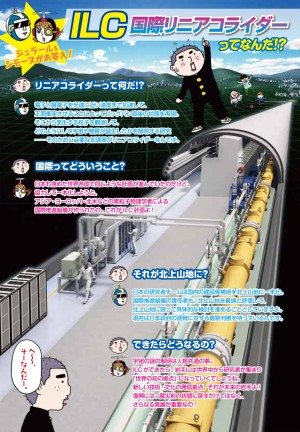
\includegraphics[width=\paperwidth]{figures/Iwatecomics.jpg}};
 % \tikz\node[opacity=0.2]{\centering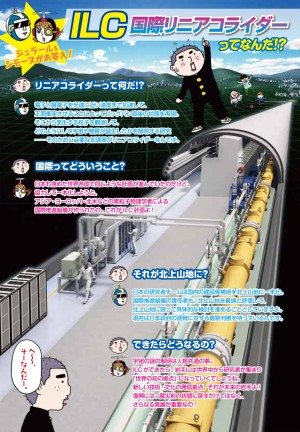
\includegraphics[height=\paperheight]{figures/Iwatecomics.jpg}};
 }
\begin{frame}
  \titlepage
\end{frame}
}
\setcounter{tocdepth}{2}
\begin{frame}{Table of contents}
  \tableofcontents
\end{frame}

%---------------------------------------------------------------------------------------------------------

\section{New beam parameter sets for the ILC250 stage}

\begin{frame}{ILC250 Beam Parameter Sets}
At AWLC17 at SLAC, the ILC250 beam parameters were suggested to be changed in order to \textbf{increase the luminosity}.\\
{\small Yokoya: \url{https://agenda.linearcollider.org/event/7507/contributions/39290/attachments/31821/47993/HigherLumi250GeV-AWLC2017-Yokoya.pdf}}\\
In the current CR, set (A) was selected as the new parameter scheme.
 \begin{table}
\label{tab:Parameters}
\centering
\begin{tabularx}{0.55\textwidth}{llll}
\hline\hline
\textbf{Set}  & \textbf{$\epsilon_x$ [\murm m]} & \textbf{$\beta_x$ [mm]} & \textbf{$\beta_y$ [mm]}\\
\hline
\cline{1-4}
\hline
 TDR & 10 & 13.0 & 0.41\\
 \alert{(A)} & 5 & 13.0 & 0.41\\
 (B) & 5 & 9.19 & 0.41\\
 (C) & 5 & 9.19 & 0.58\\
\hline\hline
\end{tabularx}
\end{table}
\alert{Caveat:\\
Reducing the emittance leads to stronger beam-beam interactions, and therefore to increased \positron \electron pair background.}
\end{frame}
%--------------------------------------------------------------------------------------------------------------
\AtBeginSection[] {
  \begin{frame}<beamer>
     \tableofcontents[currentsection,
     currentsubsection,
     %hideothersubsections,
     subsectionstyle=show/shaded/hide,
     subsubsectionstyle=show/show/hide]
  \end{frame}
}
%--------------------------------------------------------------------------------------------------------------
\section{Pair background density}
\begin{frame}{Background event generation using GuineaPig}
GuineaPig acc.dat file:\\
{\small\texttt{\textcolor{Gray}{\$ACCELERATOR:: ILC-250GeV-SetC \\                                                                            
\{energy=125.0;particles=2.0;charge\_sign=-1;\\
f\_rep=10.0;n\_b=1312;\\}
beta\_x=9.19;beta\_y=0.58;\\
emitt\_x=5.0;\textcolor{Gray}{emitt\_y=0.035;\\
sigma\_z=300.0;scale\_step=1.0;\\
waist\_x=240;waist\_y=240;\\
espread.1=0.00188;espread.2=0.00152;which\_espread=3;\}}
}}\\
\vspace*{0.3cm}
 The background generation in GuineaPig \alert{does not include a crossing angle}!\\
 The crossing angle is applied later on in the Geant4 simulation of the SiD detector.
\end{frame}

\begin{frame}{Pair background density in a 5\,T solenoid field}
\sidlogo
Calculating the path of the pairs deflected in the magnetic field
\begin{tikzpicture}
\node [anchor=west] (pipe) at (-1,3) {\Large Beam pipe};
\begin{scope}[xshift=1.5cm]
    \node[anchor=south west,inner sep=0] (image) at (0,0) {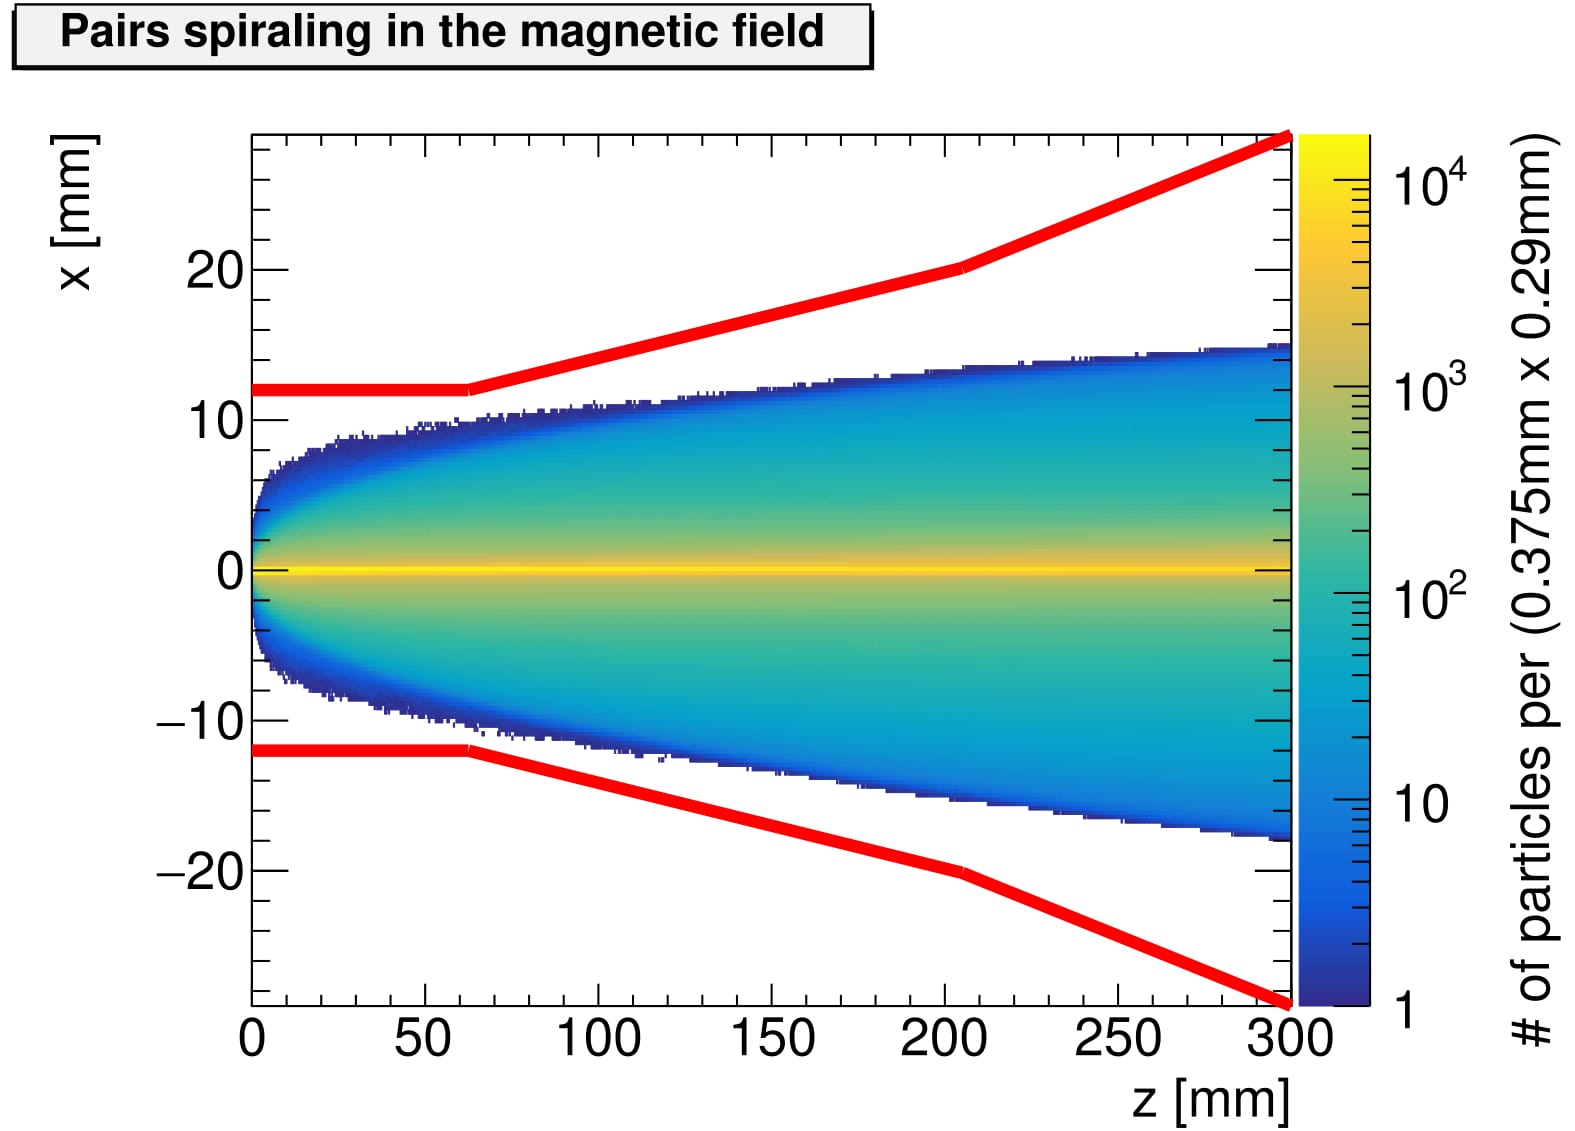
\includegraphics[width=0.7\textwidth]{ILC250_figures/Helix_tracks_xz_100bunches_250GeV_5T_DanielJeans-1.jpg}};
    \begin{scope}[x={(image.south east)},y={(image.north west)}]
        \draw [-latex, ultra thick, red] (pipe) to[out=0, in=-120] (0.3,0.65);
    \end{scope}
\end{scope}
\end{tikzpicture}%
\end{frame}


\begin{frame}{Pair background density in a 5\,T solenoid field}
\sidlogo
 \begin{figure}
\centering
\begin{subfigure}[t]{0.35\textwidth}
\centering
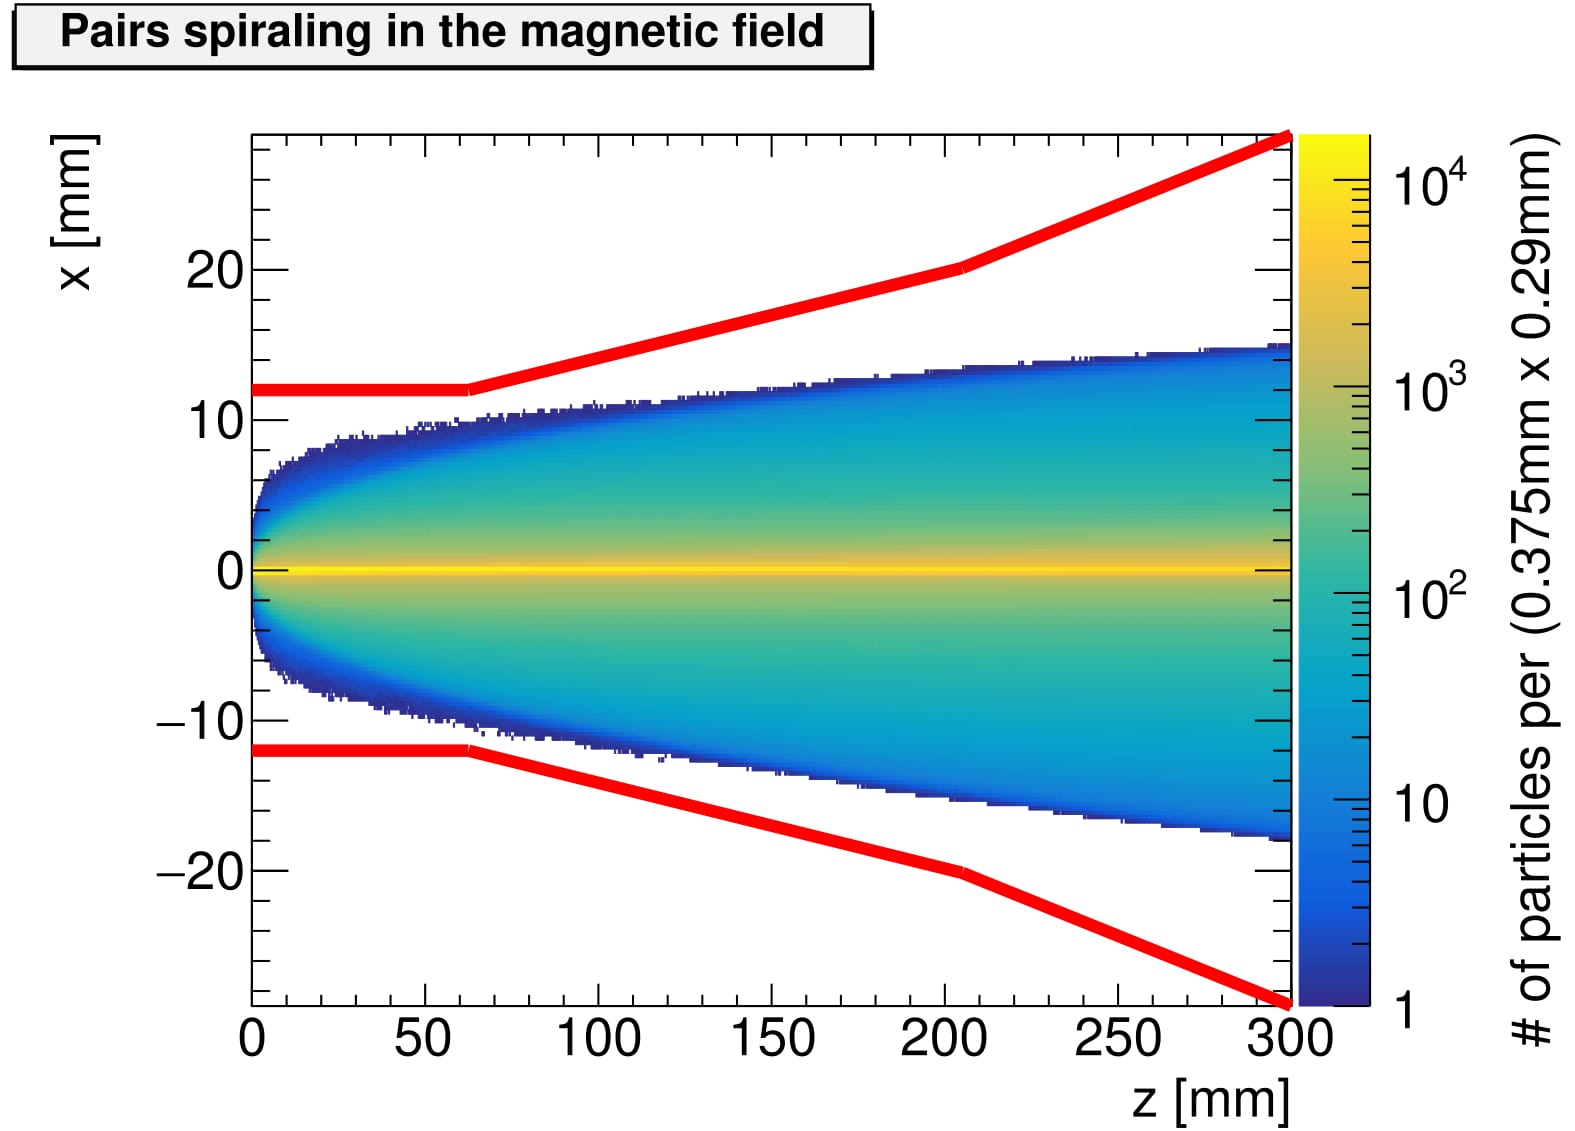
\includegraphics[width=\textwidth]{ILC250_figures/Helix_tracks_xz_100bunches_250GeV_5T_DanielJeans-1.jpg}
\caption{ILC250 set (TDR)}
\end{subfigure}
\hspace*{0.1cm}
\begin{subfigure}[t]{0.35\textwidth}
\centering
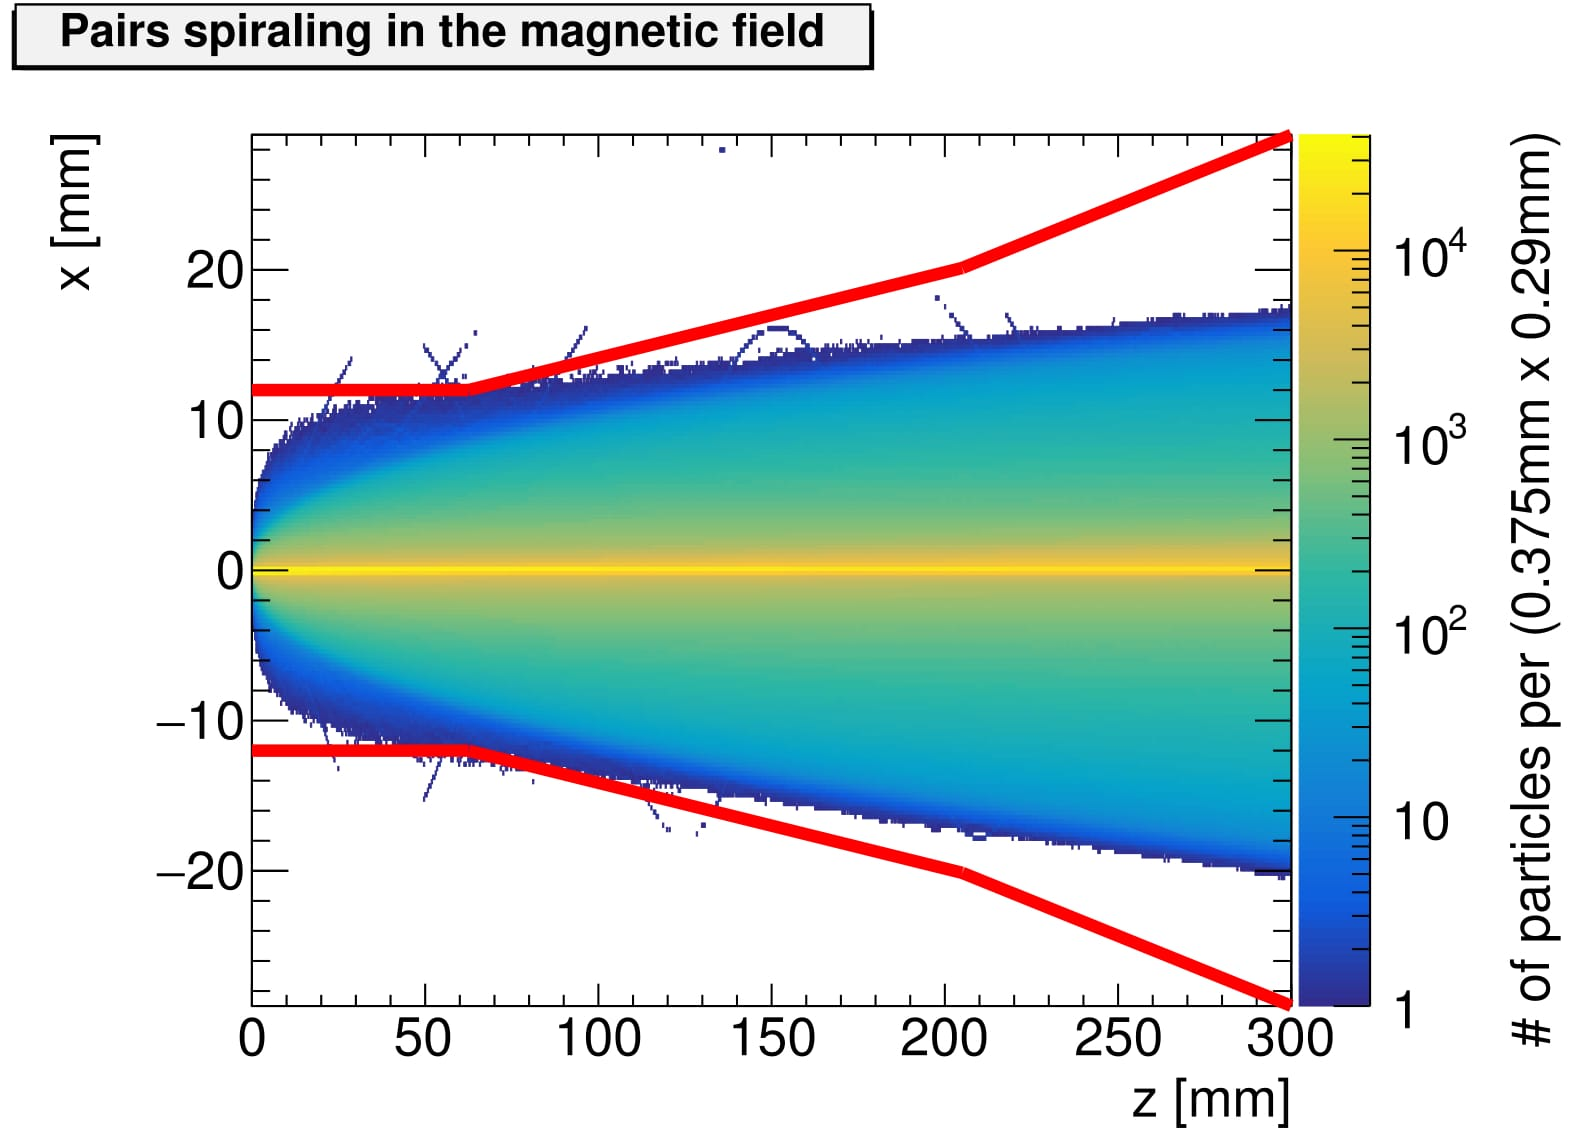
\includegraphics[width=\textwidth]{ILC250_figures/Helix_tracks_xz_80bunches_250GeV_5T_Reduced_Emittance_x-1.jpg}
\caption{ILC250 set (A)}
\end{subfigure}
\\
\begin{subfigure}[t]{0.35\textwidth}
\centering
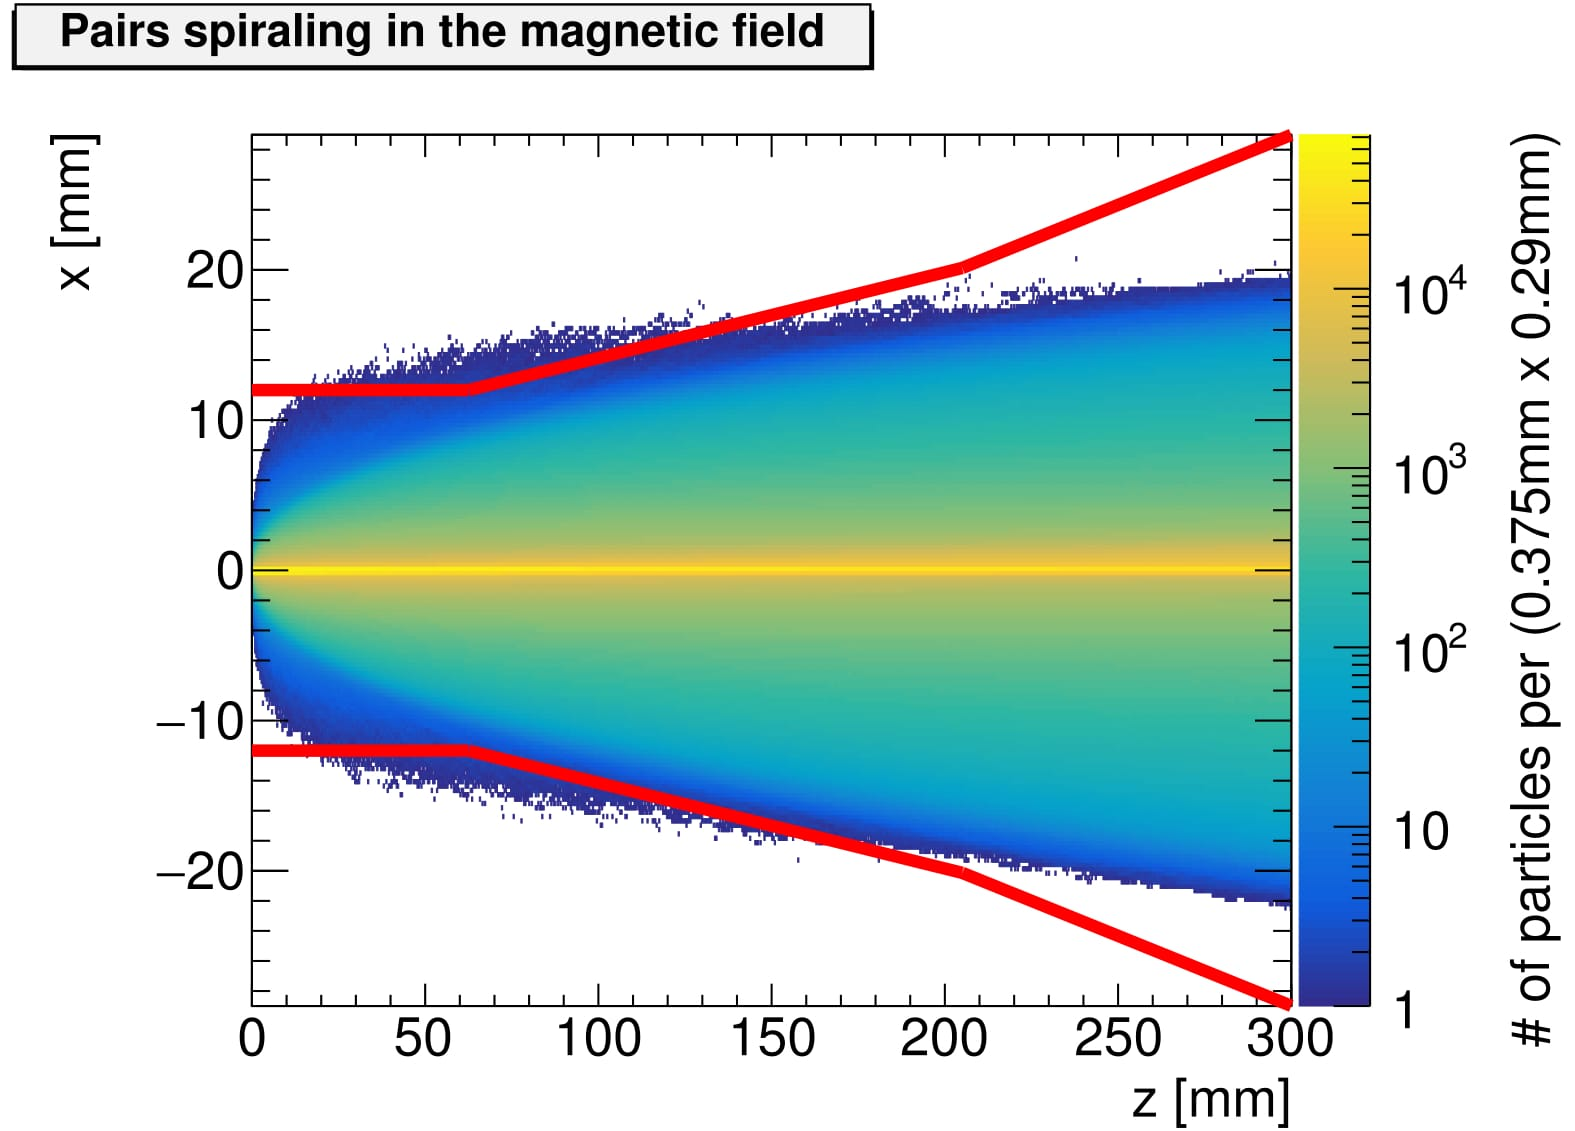
\includegraphics[width=\textwidth]{ILC250_figures/Helix_tracks_xz_50bunches_250GeV_5T_Reduced_Emittance_x_Reduced_Beta_x-1.jpg}
\caption{ILC250 set (B)}
\end{subfigure}
\hspace*{0.1cm}
\begin{subfigure}[t]{0.35\textwidth}
\centering
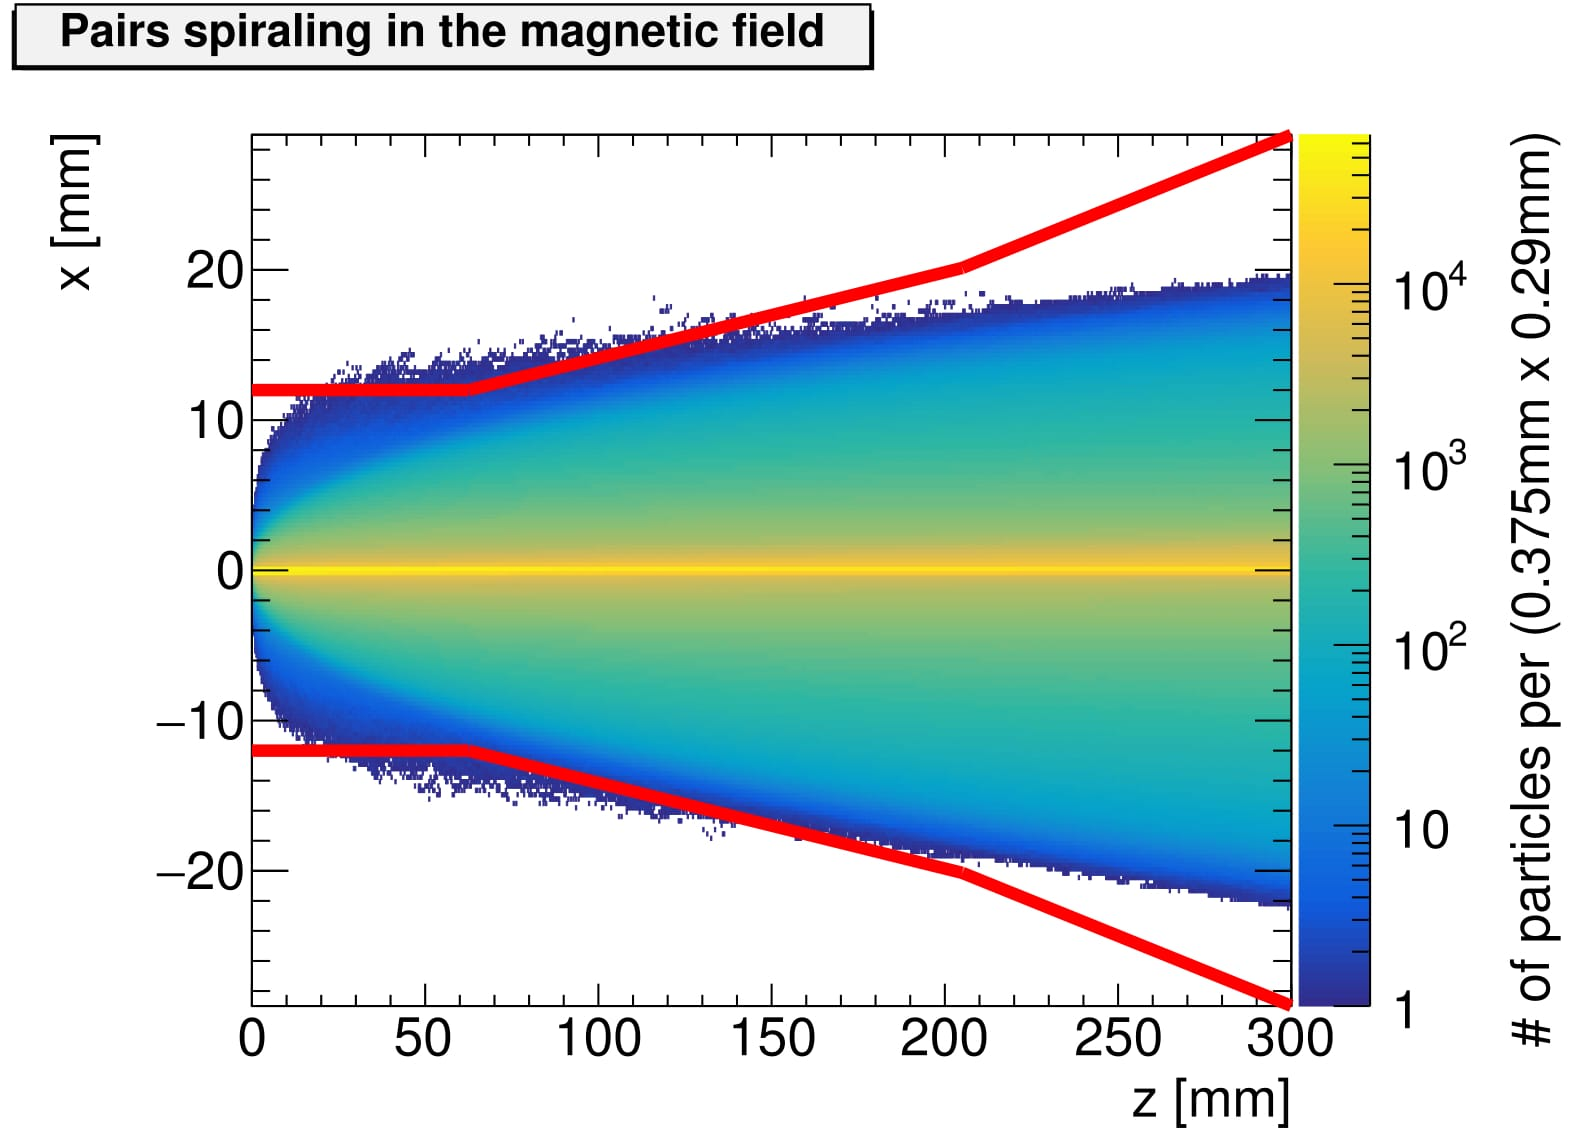
\includegraphics[width=\textwidth]{ILC250_figures/Helix_tracks_xz_50bunches_250GeV_5T_Reduced_Emittance_x_Reduced_Beta_x_Increased_Beta_y-1.jpg}
\caption{ILC250 set (C)}
\end{subfigure}
\caption{Pair background density for the different ILC250 beam parameter sets.
The beam pipe is represented by the red solid lines.}
\label{fig:Envelopes}
\end{figure}

\end{frame}

\begin{frame}{Projection of the pair background density along x}
\sidlogo
\begin{center}
 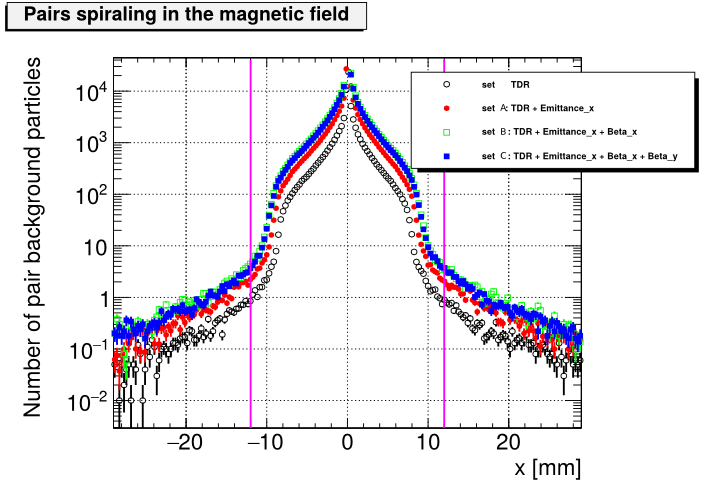
\includegraphics[width=0.72\textwidth]{ILC250_figures/HelixEnvelope_Projection_Comparison_250GeV_parametersets_NEWSETNAMES.png}
\end{center}
The envelopes are in all schemes well contained within the beam pipe. Less than 10 particles per bunch crossing are to be expected outside the beam pipe.
\end{frame}

\section{SiD Occupancy}
\subsection{SiD design: New L*, w antiDiD}
\begin{frame}{VXD Occupancy: New L*, w antiDiD}
\sidlogo
\alert{Normalized Occupancy}: Number of cells containing a certain amount of hits, normalized by the total number of cells of the vertex detector.
 \begin{figure}
\centering
\begin{subfigure}[t]{0.48\textwidth}
\centering
\includegraphics[width=\textwidth]{ILC250_figures/Occupancy_Comparison_All_layers_wrt_cells_ILC250_Comparison_ALL_SETS_5T_w_antiDiD.png}
\caption{\alert{All layers}}
\end{subfigure}
\hspace*{0.2cm}
\begin{subfigure}[t]{0.48\textwidth}
\centering
 \includegraphics[width=\textwidth]{ILC250_figures/Occupancy_Comparison_Layer_0_numcells_ILC250_Comparison_ALL_SETS_5T_w_antiDiD.png}
 \caption{\alert{Layer 0}}
\end{subfigure}
\end{figure}
The occupancy in layer 0 for the new sets is significantly increased with respect to the TDR scheme.
\end{frame}

\begin{frame}{VXD Occupancy: New L*, w antiDiD - Dead cells}
\sidlogo
\alert{Normalized number of dead cells}: Number of cells with full buffer, normalized by the total number of cells of the vertex detector.
\begin{figure}
\centering
\begin{subfigure}[t]{0.48\textwidth}
\centering
\includegraphics[width=\textwidth]{ILC250_figures/Occupancy_Comparison_All_layers_deadcells_ILC250_Comparison_ALL_SETS_5T_w_antiDiD.png}
\caption{\alert{All Layers}}
 \end{subfigure}
\hspace*{0.2cm}
\begin{subfigure}[t]{0.48\textwidth}
\centering
 \includegraphics[width=\textwidth]{ILC250_figures/Occupancy_Comparison_Layer_0_deadcells_ILC250_Comparison_ALL_SETS_5T_w_antiDiD.png}
\caption{\alert{Layer 0}}
\end{subfigure}
\end{figure}
In layer 0, the number of cells with full buffers reaches the critical limit (10\textsuperscript{-4} of all cells).
\end{frame}
%--------------------------------------------------------------------------------------------------------------
\setcounter{tocdepth}{3}
\AtBeginSubsection[] {
  \begin{frame}<beamer>
     \tableofcontents[currentsection,
     currentsubsection,
     %hideothersubsections,
     subsectionstyle=show/shaded/hide,
     subsubsectionstyle=show/show/hide]
  \end{frame}
}
%--------------------------------------------------------------------------------------------------------------
\subsection{Comparing different SiD designs}
\begin{frame}{VXD Occupancy: Different SiD designs, Set (A)}
\sidlogo

\begin{figure}
\centering
\begin{subfigure}[t]{0.48\textwidth}
\centering
\includegraphics[width=\textwidth]{ILC250_figures/Occupancy_Comparison_All_layers_wrt_cells_ILC250_Comparison_Set_A_All_SiD_designs.png}
\caption{\alert{All layers}}
 \end{subfigure}
\hspace*{0.2cm}
\begin{subfigure}[t]{0.48\textwidth}
\centering
\includegraphics[width=\textwidth]{ILC250_figures/Occupancy_Comparison_Layer_0_numcells_ILC250_Comparison_Set_A_All_SiD_designs.png}
\caption{\alert{Layer 0}}
\end{subfigure}
\end{figure}
\normalsize SiD design with \textbf{old L* (3.5\,m) and antiDiD} shows the \textbf{lowest occupancy}.
\end{frame}

\subsection{Dependency on Phi and Z}
\begin{frame}{VXD Occupancy: Comparison of parameter sets}
\sidlogo
\alert{Normalized number of dead cells per $\Phi$ or z-bin}\footnote{$\Phi$-bin size: 2$\pi$/100 = 0.062\,rad, z-bin size: 0.5\,mm}: Number of cells with full buffer, normalized by the total number of cells of the vertex detector.
\begin{figure}
\centering
\begin{subfigure}[t]{0.48\textwidth}
\centering
\includegraphics[width=\textwidth]{ILC250_figures/Occupancy_Phi_Comparison_All_layers_deadcells1_ILC250_ALL_SETS_5T_w_antiDiD.pdf}
 \end{subfigure}
\hspace*{0.2cm}
\begin{subfigure}[t]{0.48\textwidth}
\centering
\includegraphics[width=\textwidth]{ILC250_figures/Occupancy_Phi_Comparison_All_layers_deadcells2_ILC250_ALL_SETS_5T_w_antiDiD.pdf}
\end{subfigure}
\end{figure}
No strong dependence in $\Phi$ or z. AntiDiD reduces hits from pairs backscattering from the BeamCal.
\end{frame}

\begin{frame}{VXD Occupancy: Different SiD designs, Set (A)}
\sidlogo
\begin{figure}
\centering
\begin{subfigure}[t]{0.48\textwidth}
\centering
\includegraphics[width=\textwidth]{ILC250_figures/Occupancy_Phi_Comparison_All_layers_deadcells1_ILC250_Set_A_All_SiD_designs.pdf}
 \end{subfigure}
\hspace*{0.2cm}
\begin{subfigure}[t]{0.48\textwidth}
\centering
\includegraphics[width=\textwidth]{ILC250_figures/Occupancy_Phi_Comparison_All_layers_deadcells2_ILC250_Set_A_All_SiD_designs.pdf}
\end{subfigure}
\end{figure}
Comparing the different SiD designs, the meaning of the antiDiD becomes more clear.\\
Again, the SiD design with the old L* yields smaller occupancies.
\end{frame}

\section{Conclusion}
\begin{frame}
\sidlogo
 According to the shown studies of the background density and the SiD occupancy for the new ILC250 parameter sets,\\
 \alert{SiD is confident that the increased occupancy can be accommodated in the design of the Vertex Detector.}\\
 \textbf{The SiD Optimization Group gives green light for the current Change Request, and welcomes the efforts on increasing the luminosity for the ILC250 stage.}\\
 \vspace*{0.5cm}
 Further studies are ongoing:
 \begin{itemize}
  \item Increased beam pipe and VXD radius
  \item Smaller VXD pixel size
  \item Effects on various physics processes
 \end{itemize}

\end{frame}


%---------------------------------------------------------------------------------

\section*{The end}
{
\usebackgroundtemplate{
 \tikz\node[opacity=0.1]{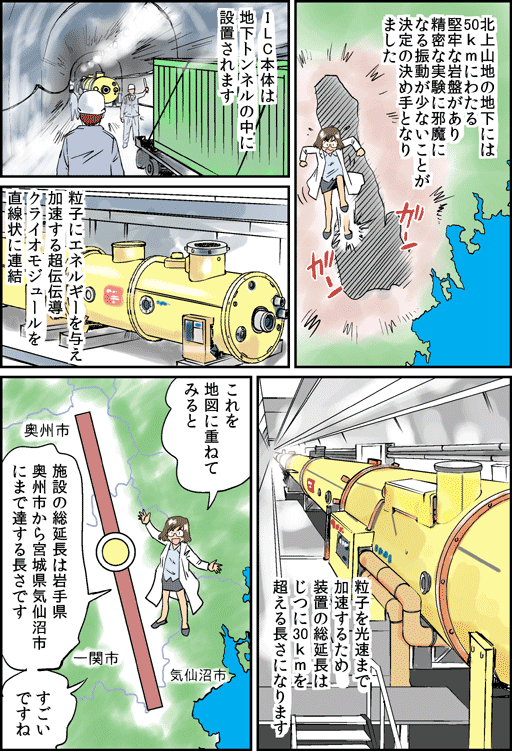
\includegraphics[width=\paperwidth,resolution=200]{figures/ilc-Comic.png}};
 % \tikz\node[opacity=0.2]{\centering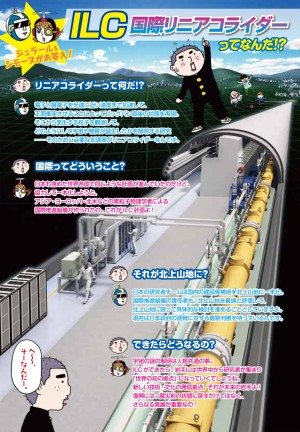
\includegraphics[height=\paperheight]{figures/Iwatecomics.jpg}};
 }
\begin{frame}
\ilclogo
\begin{center}
\textcolor{RubineRed}{
	\LARGE Thanks!\\
}
\end{center}
\end{frame}
}

\section*{References}
\begin{thebibliography}{9}
\setbeamertemplate{bibliography item}[text]
\begin{frame}{References for the Pair background study}
\tiny
\bibitem{AWLC_Yokoya}
\bibitem{AWLC_Jeans}
\bibitem{TDR1} T. Behnke, et al., \emph{The International Linear Collider - Technical Design Report, Volume 1}, 2013.
\end{frame}
\end{thebibliography}

%--------------------------------------------------------------------------------
\appendix

\begin{frame}
\begin{center}
\LARGE Additional Material
\end{center}
\end{frame}

\section{The ILC beam parameters}
\begin{frame}{ILC baseline parameters}
\ilclogo
\begin{center}
	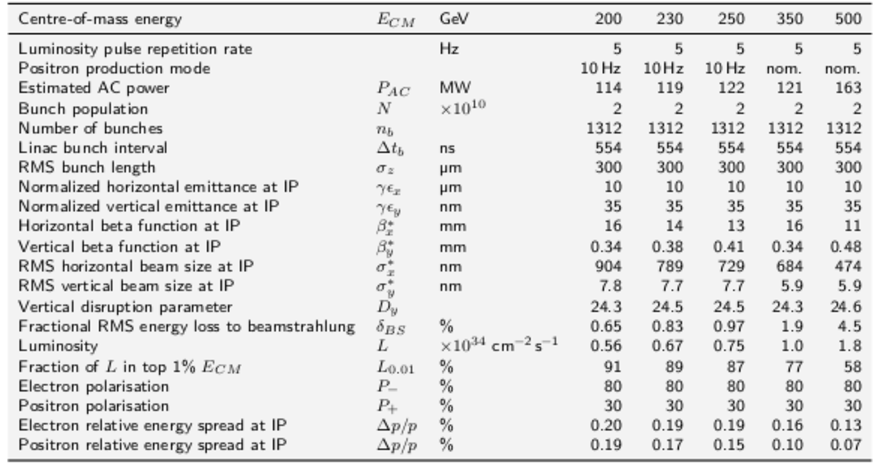
\includegraphics[width=\textwidth]{figures/ILCTDR-VOLUME_3-PART_II_ILCparameters.pdf}
\end{center}
\end{frame}
\begin{frame}{ILC parameters for the different upgrade stages}
\ilclogo
\begin{center}
	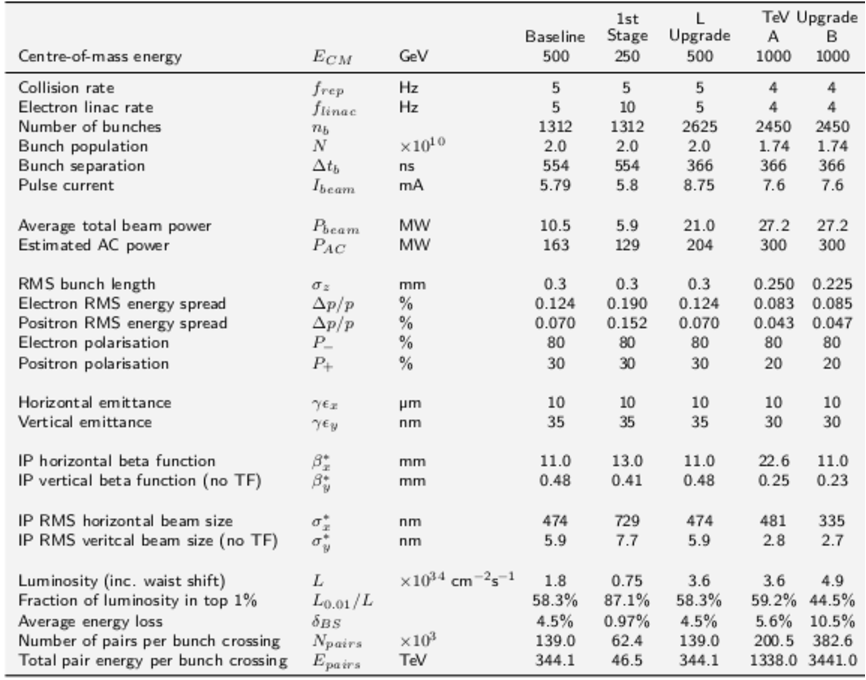
\includegraphics[width=0.8\textwidth]{figures/ILCTDR-VOLUME_3-PART_II_ILCparametersUpgrades.pdf}
\end{center}
\end{frame}

\section{Comparing different SiD designs}
\begin{frame}{VXD Occupancy: Different SiD designs, all layers}
\sidlogo
\begin{center}
\footnotesize old L*, w/o antiDiD \hfill old L*, w antiDiD \\
\includegraphics[width=0.44\textwidth]{ILC250_figures/Occupancy_Comparison_All_layers_wrt_cells_ILC250_Comparison_ALL_SETS_5T_old_LStar.png}\hfill
\includegraphics[width=0.44\textwidth]{ILC250_figures/Occupancy_Comparison_All_layers_wrt_cells_ILC250_Comparison_ALL_SETS_5T_old_LStar_w_antiDiD.png}\\
new L*, w/o antiDiD  \hfill new L*, w antiDiD\\
\includegraphics[width=0.44\textwidth]{ILC250_figures/Occupancy_Comparison_All_layers_wrt_cells_ILC250_Comparison_ALL_SETS_5T.png}\hfill
\includegraphics[width=0.44\textwidth]{ILC250_figures/Occupancy_Comparison_All_layers_wrt_cells_ILC250_Comparison_ALL_SETS_5T_w_antiDiD.png}
\end{center}
\end{frame}
\begin{frame}{VXD Occupancy: Different SiD designs, layer 0}
\sidlogo
\begin{center}
\footnotesize old L*, w/o antiDiD \hfill old L*, w antiDiD \\
\includegraphics[width=0.44\textwidth]{ILC250_figures/Occupancy_Comparison_Layer_0_numcells_ILC250_Comparison_ALL_SETS_5T_old_LStar.png}\hfill
\includegraphics[width=0.44\textwidth]{ILC250_figures/Occupancy_Comparison_Layer_0_numcells_ILC250_Comparison_ALL_SETS_5T_old_LStar_w_antiDiD.png}\\
new L*, w/o antiDiD  \hfill new L*, w antiDiD\\
\includegraphics[width=0.44\textwidth]{ILC250_figures/Occupancy_Comparison_Layer_0_numcells_ILC250_Comparison_ALL_SETS_5T.png}\hfill
\includegraphics[width=0.44\textwidth]{ILC250_figures/Occupancy_Comparison_Layer_0_numcells_ILC250_Comparison_ALL_SETS_5T_w_antiDiD.png}
\end{center}
\end{frame}

\end{document}
